\subsection{Data selection and $\gamma$-ray flux extraction}
Photon data with the latest reconstruction version (P8R2 ULTRACLEANVETO V6) of the telescope where the
observation duration takes around 9 years (starts from 7 August 2008 to 16 October 2017).
The energy range of photon is selected from 10 GeV
to 1 TeV. The upper zone of earth's limb region could be determine by
nadir angle from 68.4 to 70.0 where the coordinate figure has demonstrated in figure
\ref{gamma_production_schematic}.

\begin{figure}[h!]
    \centering
    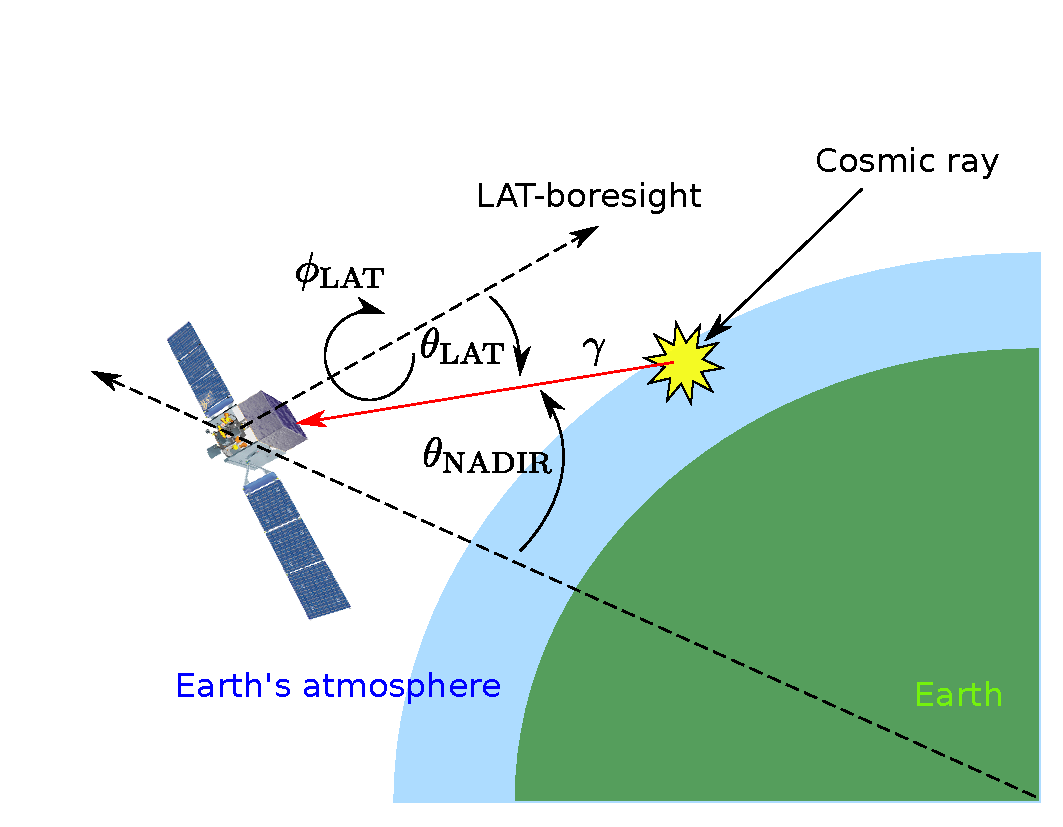
\includegraphics[width=0.6\textwidth]{img/gamma_production_schematic}
    \caption{Schematic of $\gamma$-ray production}
    \label{gamma_production_schematic}
\end{figure}

The observed flux is defined as differential flux where the governing equation
for the calculation is represented as equation (\ref{flux_definition})
\begin{equation}
    \textbf{Flux} \equiv \frac{dN_\gamma}{dE} = \frac{\int_{\textrm{Limb region}}(\textrm{Count map}/\textrm{Exposure map})}{\Delta\Omega\Delta E }
    \label{flux_definition}
\end{equation}
Where count map is filled up with selected $\gamma$-ray and exposure map represent 
the exposure time as well as effective area of spacecraft where the angle of incident
CR has taken into account.
Procedure of computation is begin with the requirement of 25 bins of histogram of
the $\gamma$-ray flux which contain a various median of energy in each bin.
Consequently, the number of count map and exposure map will be exactly the same as
the energy bins. The calculation of exposure map is done by using log file of the
spacecraft combine with the responsiveness of the spacecraft which has to be consider
in every step time while spacecraft is online. In addition, every step time of spacecraft
require the coordinate transformation which cause a huge amount of computing process.
That is the reason why paralleling processing with Master-Slave technique is applied in this work.



\subsection{Interaction model}

Incident proton spectrum in rigidity s

In this work, we use the scattering amplitude from hadronic collision \cite{K&Omodel} that could produce a photon as a secondary product that could be detected by \textit{Fermi}-LAT.
\begin{equation}
    \frac{dN_{\gamma}}{dE_\gamma}(E_\gamma)
    \propto \sum_{E_{\textrm{inc,i}}}
    % \left[\frac{E_{\text{inc,i}}}{E_{\gamma}}\Delta(E_{\textrm{inc,i}}) \right]
    % \left[ f_{pp}\textcolor{red}{\frac{dN_\textrm{H}}{dE_{\textrm{inc}}}(E_{\textrm{inc,i}})}\left\{ 1+\textcolor{olivegreen}{\frac{\sigma_{\textrm{HeN}}}{\sigma{pN}}}\left(\textcolor{red}{\frac{dN_{\textrm{H}}}{dR}}\right)^{-1} \textcolor{blue}{\frac{dN_{\text{He}}}{dR}} \frac{dR_{\textrm{He}}}{dR_{\textrm{H}}}  \right\}\right]
\end{equation}


\subsection{Optimization}


